\chapter{Introduction and Asymptotic Analysis}

CS 240 is about storing and querying data efficiently. Almost every topic in the
course follows the same pattern: define an \emph{abstract data type} (ADT) by the
operations it supports, give several \emph{implementations}, and compare them by
the running time and space of each operation. This first module sets up the
language we use to make such comparisons.

\section{Problems, Algorithms and Programs}

\begin{definition}
A \emph{problem} is a description of the relationship between inputs and outputs.
A \emph{problem instance} is one particular input. The \emph{size} of an instance,
written $n$, is a positive integer measuring how big the input is (usually the
number of items).
\end{definition}

\begin{definition}
An \emph{algorithm} is a finite, step-by-step procedure that solves every instance
of a problem. A \emph{program} is an implementation of an algorithm in a
particular programming language.
\end{definition}

Given a problem we want to (1) design an algorithm, (2) argue it is correct, and
(3) analyse its efficiency, before ever writing a program. We compare algorithms
by their resource usage as a function of $n$: \emph{running time} and
\emph{auxiliary space}.

\section{The RAM Model}

Timing a program on a real machine depends on the hardware, compiler, and load.
Instead we count operations in an idealised machine.

\begin{definition}[Random Access Machine]
The RAM model has an unbounded set of memory cells, each holding one ``word''
(a number or pointer of reasonable size). Any cell can be read or written in
constant time, and each \emph{primitive operation} (arithmetic, comparison,
assignment, following a pointer, array indexing, function call/return) takes
constant time.
\end{definition}

The running time of an algorithm on an input $I$ is then the number of primitive
operations it performs, $T(I)$. The space is the maximum number of memory cells
used beyond the input.

\begin{remark}
The RAM model assumes words have $\Theta(\log n)$ bits; it does not let us pack an
unbounded amount of information into one word. This matters for the lower bounds
later in the course and is why radix sort is not ``cheating''.
\end{remark}

\section{Asymptotic Notation}

We care about growth rate for large $n$ and ignore constant factors (which depend
on the machine anyway).

\begin{definition}[Order notation]
Let $f, g : \N \to \R_{\ge 0}$.
\begin{itemize}
  \item $f(n) \in \bigO(g(n))$ if there exist $c > 0$ and $n_0 > 0$ such that
        $f(n) \le c\, g(n)$ for all $n \ge n_0$. (Asymptotic upper bound.)
  \item $f(n) \in \Omega(g(n))$ if there exist $c > 0$, $n_0 > 0$ with
        $f(n) \ge c\, g(n)$ for all $n \ge n_0$. (Asymptotic lower bound.)
  \item $f(n) \in \Theta(g(n))$ if there exist $c_1, c_2 > 0$, $n_0$ with
        $c_1 g(n) \le f(n) \le c_2 g(n)$ for all $n \ge n_0$. (Tight bound.)
  \item $f(n) \in o(g(n))$ if for \emph{every} $c > 0$ there is $n_0$ with
        $f(n) < c\, g(n)$ for all $n \ge n_0$. (Strictly smaller growth.)
  \item $f(n) \in \omega(g(n))$ if for every $c > 0$ there is $n_0$ with
        $f(n) > c\, g(n)$ for all $n \ge n_0$. (Strictly larger growth.)
\end{itemize}
\end{definition}

Note the quantifier difference: for $\bigO$ we get to \emph{choose} one $c$; for
$o$ the inequality must hold for \emph{all} $c$.

\begin{center}
\begin{tikzpicture}[x=0.65cm,y=0.22cm]
  \begin{scope}
  \draw[-{Stealth}] (0,0) -- (7.5,0) node[right,font=\scriptsize]{$n$};
  \draw[-{Stealth}] (0,0) -- (0,19);
  \draw[very thick,blue!60!black,dashed,domain=0:7,samples=40] plot (\x,{0.35*\x*\x}) node[right,font=\scriptsize]{$c\,g(n)$};
  \draw[very thick,red!70!black,domain=0:7,samples=40] plot (\x,{3+0.5*\x+0.1*\x*\x}) node[right,font=\scriptsize]{$f(n)$};
  \draw[densely dotted] (4.6,0) node[below,font=\scriptsize]{$n_0$} -- (4.6,10.4);
  \node[font=\scriptsize] at (3.5,20.5) {$f(n) \in \bigO(g(n))$};
  \end{scope}
  \begin{scope}[xshift=7.2cm]
  \draw[-{Stealth}] (0,0) -- (7.5,0) node[right,font=\scriptsize]{$n$};
  \draw[-{Stealth}] (0,0) -- (0,19);
  \fill[green!10,domain=4.6:7,samples=30] plot (\x,{0.35*\x*\x}) -- plot[domain=7:4.6] (\x,{0.12*\x*\x}) -- cycle;
  \draw[very thick,blue!60!black,dashed,domain=0:7,samples=40] plot (\x,{0.35*\x*\x}) node[right,font=\scriptsize]{$c_2\,g(n)$};
  \draw[very thick,red!70!black,domain=0:7,samples=40] plot (\x,{3+0.5*\x+0.1*\x*\x}) node[right,font=\scriptsize]{$f(n)$};
  \draw[very thick,blue!60!black,dashed,domain=0:7,samples=40] plot (\x,{0.12*\x*\x}) node[right,font=\scriptsize]{$c_1\,g(n)$};
  \draw[densely dotted] (4.6,0) node[below,font=\scriptsize]{$n_0$} -- (4.6,10.4);
  \node[font=\scriptsize] at (3.5,20.5) {$f(n) \in \Theta(g(n))$};
  \end{scope}
\end{tikzpicture}
\end{center}
To the right of $n_0$, $f$ stays below $c\,g$ (left), or between $c_1 g$ and
$c_2 g$ (right); what happens before $n_0$ does not matter.

\begin{example}
Show $2n^2 + 3n + 11 \in \bigO(n^2)$. For $n \ge 1$ we have $3n \le 3n^2$ and
$11 \le 11 n^2$, so $2n^2 + 3n + 11 \le 16 n^2$. Take $c = 16$, $n_0 = 1$.
\end{example}

\begin{example}
Show $n^2 \notin \bigO(n)$. Suppose $n^2 \le cn$ for all $n \ge n_0$. Then
$n \le c$ for all $n \ge n_0$, which fails at $n = \max(n_0, \ceil{c} + 1)$.
\end{example}

\subsection{The Limit Rule}

Proving bounds from the definitions is tedious; the limit rule is usually faster.

\begin{theorem}[Limit rule]
Suppose $f(n), g(n) > 0$ for large $n$ and $L = \lim_{n\to\infty} f(n)/g(n)$ exists
(possibly $\infty$). Then
\[
f(n) \in \begin{cases}
o(g(n)) & L = 0,\\
\Theta(g(n)) & 0 < L < \infty,\\
\omega(g(n)) & L = \infty.
\end{cases}
\]
\end{theorem}
The converse does not hold: the limit might not exist (e.g.\ $f(n) = n(2+\sin n)$
vs.\ $g(n) = n$, which are $\Theta$ of each other).

\begin{example}
$\log n \in o(n^\epsilon)$ for any $\epsilon > 0$: by L'H\^opital,
$\lim \frac{\ln n}{n^\epsilon} = \lim \frac{1/n}{\epsilon n^{\epsilon-1}}
= \lim \frac{1}{\epsilon n^\epsilon} = 0$. Similarly $n^k \in o(b^n)$ for any
constant $k$ and $b > 1$.
\end{example}

\subsection{Useful Properties}

\begin{itemize}
  \item Identity / transitivity: $f \in \Theta(f)$; if $f \in \bigO(g)$ and
        $g \in \bigO(h)$ then $f \in \bigO(h)$ (same for the others).
  \item $f \in \Theta(g) \iff f \in \bigO(g) \text{ and } f \in \Omega(g)$.
  \item $f \in \bigO(g) \iff g \in \Omega(f)$; $f \in o(g) \iff g \in \omega(f)$.
  \item Sums: $f + g \in \Theta(\max\{f, g\})$.
  \item Constants and logs: $\log_a n \in \Theta(\log_b n)$ for any bases $a,b>1$, so
        we write just $\log n$.
\end{itemize}

\subsection{Common Growth Rates}

\begin{center}
\begin{tabular}{lll}
\toprule
Name & Function & Doubling $n$ multiplies $T$ by\\
\midrule
constant & $\Theta(1)$ & $1$\\
logarithmic & $\Theta(\log n)$ & adds a constant\\
linear & $\Theta(n)$ & $2$\\
linearithmic & $\Theta(n \log n)$ & slightly more than $2$\\
quadratic & $\Theta(n^2)$ & $4$\\
cubic & $\Theta(n^3)$ & $8$\\
exponential & $\Theta(2^n)$ & squares it\\
\bottomrule
\end{tabular}
\end{center}

Ordering: $1 \ll \log n \ll \sqrt n \ll n \ll n \log n \ll n^2 \ll n^3 \ll 2^n \ll n!
\ll n^n$, where $\ll$ means ``is $o$ of''.

\section{Worst-, Best- and Average-Case}

The running time depends on the instance, not just $n$. Define
\begin{align*}
T^{\text{worst}}(n) &= \max\{T(I) : \text{size}(I) = n\},\\
T^{\text{best}}(n) &= \min\{T(I) : \text{size}(I) = n\},\\
T^{\text{avg}}(n) &= \frac{1}{|\mathcal I_n|}\sum_{\text{size}(I)=n} T(I).
\end{align*}
Unless stated otherwise, ``the running time'' means the worst case. Note that
$\bigO$ and worst case are independent ideas: we can give $\bigO$, $\Omega$ or
$\Theta$ bounds on any of the three functions.

\begin{important}[Common pitfall]
Saying ``algorithm $A$ is $\bigO(n^2)$ and $B$ is $\bigO(n \log n)$, so $B$ is
faster'' is not justified: $\bigO$ is only an upper bound, and $A$ might in fact
be $\Theta(n)$. To compare algorithms we need $\Theta$ bounds. Also, asymptotic
bounds say nothing about small $n$.
\end{important}

\section{Analysing Pseudocode}

The strategy: assign $\Theta(1)$ to each primitive line, multiply by the number
of loop iterations, and add. Work from the inside out. It is fine to derive a
$\Theta$ bound directly, or to find matching $\bigO$ and $\Omega$ bounds
separately (often easier).

\begin{lstlisting}
Test1(n):
  sum <- 0
  for i <- 1 to n do
    for j <- i to n do
      sum <- sum + (i - j)^2
  return sum
\end{lstlisting}

The inner body is $\Theta(1)$ and runs $n - i + 1$ times, so the total is
$\sum_{i=1}^{n} (n - i + 1) = \sum_{k=1}^{n} k = \frac{n(n+1)}{2} \in \Theta(n^2)$.

\begin{lstlisting}
Test2(A, n):
  max <- 0
  for i <- 1 to n do
    for j <- i to n do
      sum <- 0
      for k <- i to j do
        sum <- sum + A[k]
      max <- maximum(max, sum)
  return max
\end{lstlisting}

The count is $\sum_{i=1}^n \sum_{j=i}^n (j - i + 1)$. For an upper bound each
term is at most $n$, giving $\bigO(n^3)$. For a lower bound, restrict to
$i \le n/4$ and $j \ge 3n/4$: there are at least $(n/4)^2$ such pairs, each with
$j - i + 1 \ge n/2$, giving at least $n^3/32 \in \Omega(n^3)$. Hence $\Theta(n^3)$.

\begin{aside}
The ``restrict the range'' trick is the standard way to get lower bounds on
nested sums without computing them exactly: throw away terms to get a smaller
sum that is easy to bound below.
\end{aside}

\subsection{Useful Sums}

\begin{itemize}
  \item Arithmetic: $\sum_{i=1}^{n} i = \frac{n(n+1)}{2} \in \Theta(n^2)$;
        more generally $\sum_{i=1}^n i^k \in \Theta(n^{k+1})$.
  \item Geometric: $\sum_{i=0}^{n-1} r^i = \frac{r^n - 1}{r - 1}$; this is
        $\Theta(r^{n})$ if $r > 1$, $\Theta(n)$ if $r = 1$, $\Theta(1)$ if $0<r<1$.
  \item Harmonic: $H_n = \sum_{i=1}^{n} \frac1i = \ln n + \gamma + o(1) \in \Theta(\log n)$.
  \item $\sum_{i=1}^n \log i = \log n! \in \Theta(n \log n)$.
  \item $\sum_{i \ge 0} i/2^i = 2$ (used for heapify).
\end{itemize}

\section{MergeSort and Recurrences}

\begin{lstlisting}
MergeSort(A, l, r):        // sorts A[l..r]
  if r <= l then return
  m <- floor((l + r) / 2)
  MergeSort(A, l, m)
  MergeSort(A, m+1, r)
  Merge(A, l, m, r)

Merge(A, l, m, r):         // A[l..m], A[m+1..r] sorted
  copy A[l..r] into S[l..r]
  i <- l; j <- m+1
  for k <- l to r do
    if i > m then A[k] <- S[j]; j <- j+1
    else if j > r then A[k] <- S[i]; i <- i+1
    else if S[i] <= S[j] then A[k] <- S[i]; i <- i+1
    else A[k] <- S[j]; j <- j+1
\end{lstlisting}

Merge takes $\Theta(r - l + 1)$ time and uses $\Theta(n)$ auxiliary space for $S$.
The running time satisfies
\[
T(n) = \begin{cases}
T(\ceil{n/2}) + T(\floor{n/2}) + \Theta(n) & n > 1,\\
\Theta(1) & n = 1.
\end{cases}
\]
It is standard to drop floors/ceilings and solve the ``sloppy'' recurrence
$T(n) = 2T(n/2) + cn$ for $n$ a power of 2.

\paragraph{Solving by unrolling.}
\begin{align*}
T(n) &= 2T(n/2) + cn = 4T(n/4) + 2cn = 8T(n/8) + 3cn = \cdots\\
     &= 2^k T(n/2^k) + kcn.
\end{align*}
With $k = \log_2 n$: $T(n) = n\,T(1) + cn \log n \in \Theta(n \log n)$.

\paragraph{Recursion-tree view.} Level $i$ of the tree has $2^i$ subproblems of
size $n/2^i$, so each level costs $cn$; there are $\log n + 1$ levels.

\begin{center}
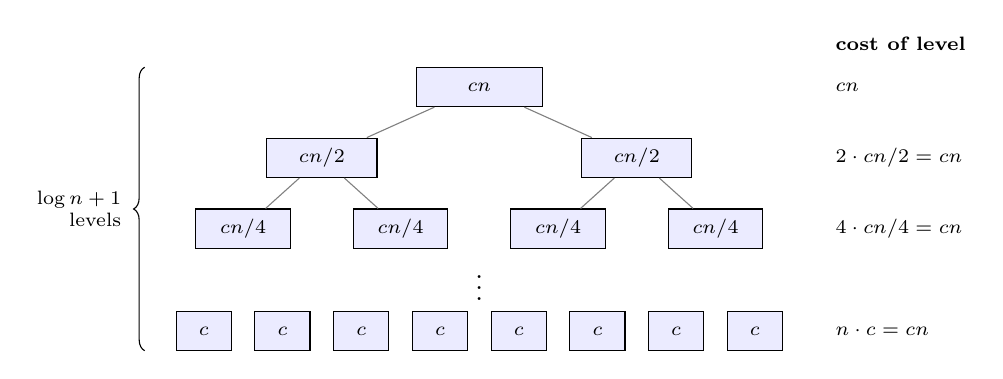
\begin{tikzpicture}[b/.style={draw,fill=blue!8,minimum height=5mm,inner sep=0pt,font=\scriptsize},
  e/.style={-,gray}]
  \node[b,minimum width=1.6cm] (r) at (4,0) {$cn$};
  \node[b,minimum width=1.4cm] (a) at (2,-0.9) {$cn/2$};
  \node[b,minimum width=1.4cm] (b) at (6,-0.9) {$cn/2$};
  \foreach \i in {0,...,3} \node[b,minimum width=1.2cm] (q\i) at (1+\i*2,-1.8) {$cn/4$};
  \draw[e] (r) -- (a); \draw[e] (r) -- (b);
  \draw[e] (a) -- (q0); \draw[e] (a) -- (q1); \draw[e] (b) -- (q2); \draw[e] (b) -- (q3);
  \node at (4,-2.45) {$\vdots$};
  \foreach \i in {0,...,7} \node[b,minimum width=0.7cm] at (0.5+\i,-3.1) {$c$};
  \foreach \y/\t in {0/{$cn$},-0.9/{$2 \cdot cn/2 = cn$},-1.8/{$4 \cdot cn/4 = cn$},-3.1/{$n \cdot c = cn$}}
    \node[font=\scriptsize,anchor=west] at (8.4,\y) {\t};
  \node[font=\scriptsize\bfseries,anchor=west] at (8.4,0.55) {cost of level};
  \draw[decorate,decoration={brace,mirror,amplitude=4pt}] (-0.25,0.25) -- (-0.25,-3.35)
    node[midway,left=5pt,font=\scriptsize,align=right] {$\log n + 1$\\levels};
\end{tikzpicture}
\end{center}
Summing $cn$ over $\log n + 1$ levels gives $\Theta(n \log n)$.

\subsection{Common Recurrences}

\begin{center}
\begin{tabular}{lll}
\toprule
Recurrence & Solution & Example\\
\midrule
$T(n) = T(n/2) + \Theta(1)$ & $\Theta(\log n)$ & binary search\\
$T(n) = 2T(n/2) + \Theta(n)$ & $\Theta(n \log n)$ & mergesort\\
$T(n) = 2T(n/2) + \Theta(\log n)$ & $\Theta(n)$ & heapify\\
$T(n) = T(cn) + \Theta(n)$, $0<c<1$ & $\Theta(n)$ & selection (expected)\\
$T(n) = 2T(n/4) + \Theta(1)$ & $\Theta(\sqrt n)$ & kd-tree range search\\
$T(n) = T(\sqrt n) + \Theta(1)$ & $\Theta(\log\log n)$ & interpolation search (avg)\\
$T(n) = T(n-1) + \Theta(n)$ & $\Theta(n^2)$ & quicksort worst case\\
$T(n) = 2T(n-1) + \Theta(1)$ & $\Theta(2^n)$ & naive recursion\\
\bottomrule
\end{tabular}
\end{center}

\begin{aside}
The Master Theorem (from CS 341) covers $T(n) = aT(n/b) + \Theta(n^d)$:
compare $d$ with $\log_b a$. In CS 240 we mostly just unroll or quote the table.
\end{aside}

\section{Summary}
\begin{itemize}
  \item Algorithms are analysed in the RAM model by counting primitive operations.
  \item $\bigO, \Omega, \Theta$ give upper, lower, tight bounds up to constants;
        $o, \omega$ are their strict versions. The limit rule is the fastest tool.
  \item Worst/best/average case is a separate choice from which bound we give.
  \item For nested loops, sum from the inside out; get lower bounds by discarding terms.
  \item MergeSort runs in $\Theta(n \log n)$ via $T(n) = 2T(n/2) + \Theta(n)$
        and uses $\Theta(n)$ extra space.
\end{itemize}
